\documentclass{report}

\usepackage{graphicx}
\usepackage{fancyhdr}

\pagestyle{fancyplain}

\lhead[\fancyplain{}{\bfseries\thepage}]
        {\fancyplain{}{\bfseries\rightmark}}
\rhead[\fancyplain{}{\bfseries\leftmark}]
        {\fancyplain{}{\bfseries\thepage}}
\lfoot[]{\fancyplain{}{\bfseries\scriptsize YardSale: The Open
        Source Point of Sale Solution}} \cfoot{}

%left margin gutter
\oddsidemargin 0.0in
%right margin gutter
\evensidemargin 1.0in
\textwidth 6.5in
%distance from bottom of top margin to top of writing
\headheight 0.0in
\topmargin 0.0in
\textheight 8.5in

\begin{document}

\begin{titlepage}
\vspace*{2cm}
\begin{center}

{\LARGE {\bf INTERIM REPORT}}\\
\vspace*{1cm}



\LARGE{ YardSale\\The Open Source Point of Sale Solution\\ }

%\vspace*{0.5cm}


\includegraphics{aslogic_smaller.png}

\large{{\bf A.S. Logic Systems Co.}\\Jesse Lovelace\\Adam
Parrish\\Mike Swigon\\Jay Johnston\\John Lamb\\Cameron Watts\\}

\vspace*{0.5cm}

{April 7, 2004}
\end{center}
\end{titlepage}

\tableofcontents

\chapter{Requirements Definition}

\section{Introduction}

YardSale is an open source Point of Sale system that is being
developed by A.S Logic Systems.  Current
implementations of Point of Sale systems are fraught with a number
of issues including often being extremely overpriced, difficult
to administer, dated in their functionality, and lacking necessary
operations.

The power of an open source system such as YardSale is the
open way in which it is designed.  A user of the YardSale system
can take off the shelf computer hardware (in many cases older hardware
will perform just as well) and create a point of sale with minimal
configuration.  In addition, supporting new hardware is trivial since
the YardSale interface specification is in no way hindered by
restrictive close-source licenses.

The name "YardSale" was concieved to emphasize the
versatility and simplicity of the system.  The parts of a
YardSale point of sale can be older, used hardware and
the underlying software can be completely free.

Being that YardSale is an open source project the initial
market will target small, locally owned retail
stores.  This type of market will allow for extensive on-site
research, as many of these businesses should be willing to work
with us to improve on the functionality of their existing POS
system.  In addition, because A.S. Logic has decided to take the
open source route, the software itself will be freely available to
all who wish to use it, the only expense that will come into play
is if the company wishes to enlist our services in setup,
troubleshooting, support, expansion, or customization.

However, we believe that YardSale can be easily used by
those who do not wish to purchase support contracts due to
the clear documentation and well-writen interfaces.

\section{Functional Requirements}

This section entails all of the minimal requirements set by the AS
Logic Systems development team for the Open Source Point of Sale, hereafter referred
to as YardSale.\\
\\YardSale should accomplish the
following Point of Sale operations:

\begin{itemize}
    \item {Manage Inventory}
    \begin{itemize}
    	\item {Add a product to the inventory}
	\item {Edit an existing inventory item}
	\item {Remove an inventory item}
	\item {Associate attributes such as price, quanity, and tax with an inventory item}
	\item {Search for an inventory item by various criteria}
	\item {Add an inventory item to a transaction (see Transaction)}
    \end{itemize}
    \item{Manage Customers}
    \begin{itemize}
    	\item{Add and remove customers}
	\item{Edit customer information such as phone number and address}
	\item{Associate a customer with a transaction (see Transaction)}
    \end{itemize}
    \item {Manage Employees}
    \begin{itemize}
    	\item{Add and remove employees}
	\item{Associate a level with employees such as "manager" and "sales associate"}
    \end{itemize}
    \item{Perform Point of Sale Transactions}
    \begin{itemize}
    	\item{ Allow an "seller/employee" to sell and inventory item to a "buyer/customer"  }
	\item{ Allow a customer to return an item to the seller }
	\item{ Calculate the tax on an item being sold }
    \end{itemize}
\end{itemize}

Each of these tasks is described in depth in their corresponding
sub sections. The functionality outlined above is designed to be as 
extensible as possible; with the correct implementation of these requirements
the YardSale System will support the expansion of functionality with great ease.

    \subsection{Information Management}
    YardSale will store information about all aspects of program operation
    data. The data that is stored can be broken down into four main subsections
    \begin{itemize}
	\item{Employee Data}
	\item{Customer Data}
	\item{Inventory Data}
	\item{Sales Data}
    \end{itemize}

    \subsection{Employee Data}
    For YardSale to properly manage 


    YardSale will store information about all aspects of program operation
    data. This is inclusive of Employee, Customer, Inventory, and Sales
    data. Employees shall have all pertinent contact information such
    as Name, Address, Phone Numbers, and Email address as well as an
    Employee Number and possibly a Social Security number saved as a
    record. Customer will have the same contact information stored as
    well. Inventory Items will have a Name and SKU number associated
    with every record, and other pertinent information about Items
    such as their cost, resale value, and tax rate will also be stored.
    Sale transactions shall be saved by referencing the primary key of
    each employee, customer, and inventory item sold during a transaction.

    %The goal of the database management tasks are to add, modify, and
    %delete information in the database. The database backend will run
    %on a MySQL server and all relevant data will be stored in its own
    %table or set of tables. More information on the database design
    %can be found in the database design document.

    \subsubsection{Inventory Management}
    %The inventory management system will have an interface for the
    %stock employees to enter new shipments. It will also have an
    %interface for the management employees to define new items for
    %sale. The most common use of the inventory management system will
    %be integrated into the checkout system. When customers are
    %checking out, inventory will be populated to the checkout screen
    %from the database, and then decremented on purchase from their
    %quantity in the database.

    \subsubsection{Customer Management}
    %The customer management system will work in a similar fashion to
    %the inventory management system. It will have only one level of
    %functionality though, the ability to define and update new
    %customer data. There will also be a small interface with the
    %database during the checkout of a customer which will allow for
    %the selection of a customer from the customer table.

    \subsubsection{Employee Management}
    %The employee management system here again will also function
    %similarly to the previous two in that it has hooks into the
    %database for employees. It will allow an authorized user the
    %ability to add and modify employee information as well as
    %disable employee accounts.\\

    Among the more specific functionality of each of these sections
    will be to allow the user to retrieve any item stored in either
    inventory, customer, or employee tables given a search
    criteria.

    \subsection{Transactions}

    Transactions are the key to any point of sale system.  The obvious
    function that a point of sale should perform is selling an item.
    However, selling an item is not simply adding up a price.  Most sales
    require information about what is being sold, who is selling it, and to whom
    the items are being sold.  These attributes are contained in a YardSale
    transaction.

    YardSale will create a transaction which contains one or more items
    either being sold or returned.  Each transaction will have an employee
    and a customer associated with it.  Since tax is extremely important
    to any transaction, tax must be added to each item since different
    items require different taxes as mandated by local, state, and national
    goverment.

    Once a transaction is created, it must be stored by the information
    management system so that a record of the transaction can be
    recalled for returns and reports.

    \subsection{Reporting}
    There will be a wide variety of reporting features available also
    as a result of the database backend. The following basic reporting
    functionality will be available in the first iteration of
    YardSale.

    \begin{itemize}
        \item{Payroll for Employees}
        \item{Top Sales for Inventory Items}
        \item{Top Sales for Employees}
        \item{Top Sales for Customer}
        \item{Revenue Reporting given any time frame}
        \item{Hourly Employee Log Reporting}
    \end{itemize}

    All of the reports will be output to a pdf via \LaTeX type
    setting. This will provide ease of portability and a wide range of
    flexibility in reporting.

    \subsection{User Level Access Rights}
    YardSale has three different levels of user interactivity. There
    are Managers, Sales Associates, and Administrative users.

    \subsubsection{Sales Associate Functionality}
    Sales associates are likely going to be the primary users of the
    YardSale system. However they will have a limited set of
    functionality when they login. Their privileges will be limited to
    basic customer management and transaction processing. They have no
    real need for full inventory capabilities nor do they need the
    ability to manage or browse employee information.

    When a sales associate logs into YardSale they will see the following options:

    \begin{itemize}
        \item Transaction Processing
        \item Customer Management
    \end{itemize}

    \subsubsection{Manager Functionality}
    The managers primary function in YardSale is to make sure that all
    of the inventory items, customers, and employees are correctly
    maintained. They are also the only primary user on the system
    allowed to run reporting functions.

    When a manager logs in to YardSale they will have a full set of
    functionality available to them from the main screen inclusive of
    the following:

    \begin{itemize}
        \item Inventory Management
        \item Transaction Processing
        \item Customer Management
        \item Employee Management
        \item Reporting
    \end{itemize}

    \subsubsection{Administrative Functionality}

    The administrative user is basically a built in manager user. This
    user will have full rights to the system and the password will be
    able to unlock other accounts in the system that are locked due to
    loss of password. The administrative user will likely never be
    used in day to day use of YardSale, however it is provided as a
    safety to always allow the access of encrypted data in case of
    total loss of management capability.

\section{Non Functional Requirements}

    \subsection{Cross Platform}
    The YardSale software is to be developed using the wxWindows libraries for C++,
    which creates GUIs (Graphical User Interfaces) that are
    platform independent.  The YardSale software will be able to
    run on any major operating system on today's market.

    \subsection{Cross Architecture}
    The main purpose of the YardSale software is to be very
    independent of all architectural aspects of the system, using
    minimal system resources.  The idea is to be able to use any system
    to run the software appropriately.

\section{System Constraints}
    \subsection{Interfaces}
    The YardSale system must support the use of several peripheral interfaces
    to aid in the completion of POS transactions and other functionality outlined
    previously.  The interfaces are outlined as follows:
        \begin{itemize}
	    \item {\bf Cash Drawers} The system must support the use of a
	    cash drawer for storage of money exchanged during transactions.
	    It shall pop open upon the completion of a transaction or when 
	    prompted by the user.

	    \item {\bf Magnetic Card Scanners} The system must support the use
	    of a magnetic card scanner for automatic input of information.  These
	    scanners must correctly input information stored on both credit cards
	    and employee access cards.

	    \item {\bf Barcode Scanners} The system must support the use of
	    a barcode scanner for automatic input of items for inventory
	    and transaction processing.

	    \item {\bf Receipt Printers} The system must support the use of
            a receipt printer.  The printers must print specified information
            at the conclusion of each transaction and will also be used with
	    the reporting functionality.

            \item {\bf TouchScreen Monitor} The system must support the use
            of TouchScreen monitors.  The monitor shall act as both input and
	    output devices for the system.  The monitors must correctly read 
            the commands given and relay them to the system.

\section{External Dependencies and Interfaces}

\section{Preliminary Design}

    \subsection{Major Modules}

        \subsubsection{Database}
        The Database module works as the translator between
        the user interface and the database.  It converts calls
        made by the GUI into SQL queries to be sent to the
        database.  When the query results are returned from the
        database,the Database converts these items to a
        Database Type (discussed in next section) to be read by the
        GUI. OTL Libraries will be used in conjunction with ODBC to
    provide database connectivity with the user interface. OTL is
    a cross platform library for ODBC.
        \subsubsection{Database Types}
        The Database Types module is the superclass for all information that
        may be sent to the GUI from the database.  It contains
        function calls for each of the following types:
        \begin{list}{}
            \item{{\bf Inventory Type:} contains variables for all
            possible inventory management items stored in the
            database.  Coordinates with the Inventory Management
            view in the GUI, which is also used by Transactions.}
            \item{{\bf Customer Type:} contains variables for
            all possible customer management items stored in the database.
            Coordinates with the Customer view in the GUI,
            which is also used by Transactions.}
            \item{{\bf Employee Type:} contains variables for
            all possible employee management items stored in the
            database.  Coordinates with the Employee Management
            view in the GUI.}
            \item{{\bf Yard Transaction:} contains variables for all
            possible transaction items stored in the database.
            Coordinates with the Transaction view in the GUI.}
        \end{list}{}
        \subsubsection{GUI wxWindows}
        The GUI wxWindows module defines all interfaces used by the
        GUI.  It contains functions derived from the wxWindows
        libraries for C++.  It also interacts with the
        Database module to display information sent from the
        database.\\

        \newpage


    \subsection{System Architecture}

    The figure shown below outlines the class dependencies and hierarchy of
    the modules described in section 1.5.1.\\

    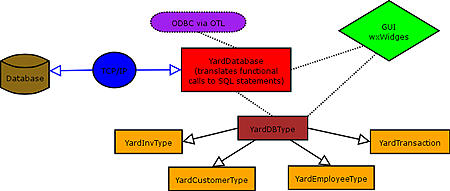
\includegraphics{yardsale_modules.png}\\
    %\caption{System Architecture Flow Chart}

\section{Preliminary Project Task Plan}
    %Scope and Size of Project Paragraph

    \subsection{Milestones}
    \begin{description}
        \item[2004-03-05] FEATURE FREEZE - deadline for adding functional
        features to the design of the POS.
        \item[2004-03-07] ITERATION 1 - all requirements for first
        iteration to be completed and documented in the interim
        report.
        \item[2004-04-01] ITERATION 2 - all secondary requirements
        to be completed for the second iteration.
        \item[2004-04-17] CODE FREEZE - deadline for beginning the
        coding of features; those not already implemented will be removed;
        testing only beyond this point
        \item[2004-04-27] FINAL DELIVERABLE - completion of
        prototype for presentation to the CSC department at the
        Posters and Pies event.
    \end{description}

    \subsection{Team Member Roles and Responsibilities}
    The following figure displays a graphical hierarchy of the team's
    roles:\\
    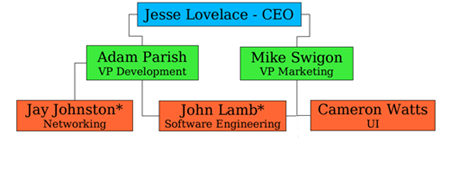
\includegraphics{organization.png}
    \\The team roles are defined as follows:

    \begin{description}
        \item[Jesse Lovelace] As the CEO of A.S. Logic Systems,
        Jesse is in charge of all aspects of the project.  Though
        he works very closely with both VPs, Jesse is the ultimate
        decision maker for the team.  In addition to his roles as
        CEO, Jesse is also in charge of the design and
        implementation of the User Interface and all security
        aspects.
        \item[Adam Parrish] Adam is the Vice President in charge
        of Development at A.S Logic Systems.  He works closely
        with both the CEO and VP of Marketing to see that
        YardSale's implementation is both correct and timely.  In
        addition to these company roles, Adam is also the lead
        Database Programmer; seeing to it that the database is
        functioning properly and creating the SQL scripts for
        populating and querying the database.
        \item[Mike Swigon] Mike is the Vice President of
        Marketing at A.S. Logic Systems.  He works closely with
        both Adam and Jesse to both design the entire system and
        to insure that its implementation is correct.  In addition
        to these responsibilities, Mike works with Adam in database
        setup and creation of SQL scripts for populating and
        querying the database.
        \item[John Lamb] John's responsibilities fall primarily in
        interfacing with the database.  He works closely with Jesse
        to develop a UI that can correctly and securely
        communicate information to and from the database; also
        implementing the SQL statements developed by Mike and
        Adam.
        \item[Jay Johnston] Jay's responsibilities fall primarily
        in creation of the UI and networking the system during
        setup.  He works closely with Jesse to develop modules
        for required functionality of the interface.
        \item[Cameron Watts] Cameron's responsibilities fall
        primarily on marketing and system research.  He works
        closely with the design group to ensure YardSale's
        functionality is top-of-the-line and user friendly.
    \end{description}


\chapter{Design}

    The following sections are related to the design of YardSale
    in regards to the database level design as well as the client
    application level design. The first section provides a high level
    explanation of the database architecture using UML diagrams. The
    following section explains design related issues of the YardSale
    client program.

\section{YardSale Database Design}

    The YardSale database was designed with security and efficiency in
    mind. The goal was, as it is in any database, to seperate unrelated
    data and key similar items together with table relations. The global
    database model is seen in the diagram on the following page. Although
    it is not necessarily easy to read the table relations can be seen, and
    table specifics like field values, indexes, and foreign and primary keys
    can be seen in the following table diagrams.

    \newpage

    {\bf YardSale Global Database Diagram}\\
    \\
    \\
    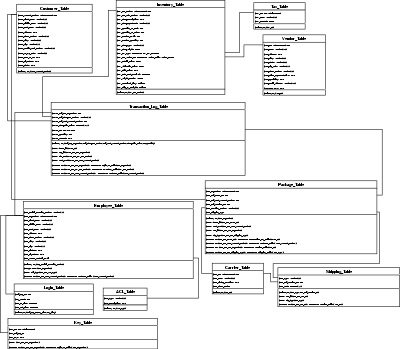
\includegraphics{Database_Layout.png}

    \newpage

        \subsection{Customer Management}

        Since customer management is basically a simple task it is maintained in only
        one table. There is no real need to have their data stored accross many
        different tables since all of the information is just personal data.

        {\bf Customer Table}\\
        \\
        \\
        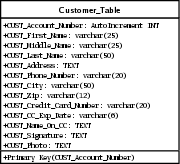
\includegraphics{Tables/CustomerTable.png}\\
        \\
        The above UML diagram shows the layout of the customer table. The object of this
        table is to manage customer personal information for later reference in
        transactions. By allowing this associativity YardSale will later be able to
        formulate reports on how much each of its customers spend for example. It also
        provides a rather in depth directory of all of a business's clients for use
        in any form they see fit.

        The data stored begins with the customer account number which is just an
        arbitrarily assigned number that is managed by the database management
        system. It is also the primary key for the table and is therefore unique.
        First, Middle, and Last names are all stored in seperate fields of their own,
        as is the Address information. Credit information can also be stored about users
        but is optional, and is also planned to be stored in the field as an encrypted
        string of data so that underprivileged users can not access it. Two interesting
        features about this table is the ability to store a link to a photograph and
        signature for each customer. That way it will aid in positively identifying a
        customer when they are checking out with check or credit.


        \newpage

        \subsection{Inventory Management}

        YardSale's Inventory Management scheme spans over three tables. The main table that
        stores actual inventory description information is the Inventory Table itself. The
        other two tables are used to support the main table. They are the Tax table and the
        Vendor Table. The tax table is basically a storage area for different tax types, and
        the Vendor Table is a storage table for Vendor information or Inventory Supplier
        information.\\
        \\
        {\bf Inventory Table}\\
        \\
        \\
        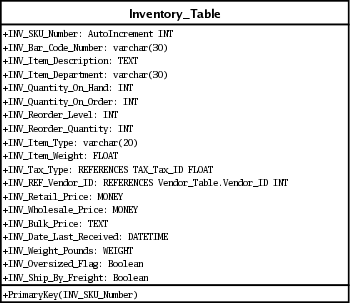
\includegraphics{Tables/InventoryTable.png}\\
        \\
        \\
        This table being the main Inventory storage structure contains all information needed
        about any inventory item. The record primary key is the SKU number which is a user
        defined number or character string. These are often used in small businesses to
        internally key their inventory. Manufacturers will often have a bar code associated
        with each item the produce as well so their is a field available for that as well.
        Each item can be briefly described, and associated with a department for further
        subcatagorizing. The number of any particular item is maintained as well as how many
        of the item are on order. There is a field for storing the number at which an item should
        be reordered, and also how many to reorder at that time. There are varying description
        fields such as item type and weight as well. Three pricing fields are supplied. The
        first two are statically maintained as retail and wholesale price. The third price
        type varies on the number of items being purchased. This field is maintained in XML
        format so that as many different pricing levels as are needed can be defined. When an
        item is received it updates the field corresponding to last received. Some items are
        oddly shaped or are overly heavy, either of these two options could cause the oversized
        flag to be set, and if the oversized flag is set a ship by freight option would also be
        set, but they are mutually exclusive and the ship by freight can be set without the
        oversized flag being set.\\
        \\
        {\bf Tax Table}\\
        \\
        \\
        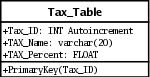
\includegraphics{Tables/TaxTable.png}\\
        \\
        \\
        The tax table is just a support table for the inventory items. It is referenced by ID
        depending on the desired taxing an item should have. Using a table allows for user definable
        tax types, and allows the database to be flexible to tax changes. All that the table needs
        is a Tax Name and a percentage for taxing items. The ID field is managed internally by the
        database management system and is also the primary key for the table.\\
        \\
        {\bf Vendor Table}\\
        \\
        \\
        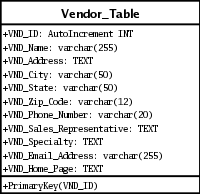
\includegraphics{Tables/VendorTable.png}\\
        \\
        \\
        The Vendor Table is used also as a supporting table for the inventory. This information
        pertains to the supplier of the items being sold. When an item reaches its reorder level
        in the Inventory Table, the information in this table would be used to make the order to
        resupply. The table is keyed by a unique ID that is managed by the database management
        system. The company name, address, and pertinent contact information is maintained along
        with a sales representative's name. There are optional fields for company specialty, email
        address, and homepage as well.

        \subsection{Transaction Handling}

        Transaction Handling is a process that has data spanning two tables with two more supporting
        tables. Transaction handling is split into two sections. The first section being the actual
        day to day transaction, and then the added functionality of packaging the items sold during
        the transaction.\\
        \\
        \\
        {\bf Transaction Table}\\
        \\
        \\
        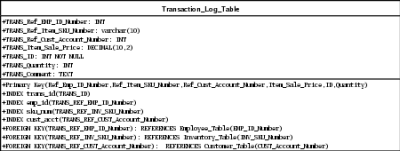
\includegraphics{Tables/TransactionLogTable.png}\\
        \\
        \\
        The Transaction Log Table is used to store information that links Customers, Employees, and
        inventory items. Each entry in the transaction table represents an item sold during a transaction.
        Since the key is not a single ID number it is the combination of the Customer, Employee, Item,
        Quantity and Price, the ID can be used to represent the overall transaction. Any row that contains
        an equivalent ID belongs to the same transaction.
        \\
        \\
        {\bf Package Table}\\
        \\
        \\
        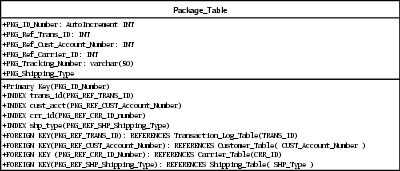
\includegraphics{Tables/PackageTable.png}\\
        \\
        \\
        The Package Table is used to store information about a package. There is a link to a transaction ID
        so that items can be associated with a package. There is also a link to a customer from the package
        table. The reason there is a link from the package table is because one customer may wish to buy
        something for another so the customer who made the transaction will not necessarily be the same as
        the one who will receive the package. There is also a reference to a carrier and a shipping type.
        A tracking number field is provided for when the tracking number is issued by the Carrier.
        \\
        \\
        {\bf Carrier Table}\\
        \\
        \\
        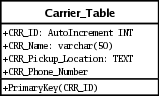
\includegraphics{Tables/CarrierTable.png}\\
        \\
        \\
        The Carrier table is a support table for the Package table. It provides information about the different
        shipping services. The information maintained here is just what is necessary to get a package shipped.
        There is a phone number, pickup location and an ID associated with each entry.
        \\
        \\
        {\bf Shipping Table}\\
        \\
        \\
        The Shipping Table is also a support table for the Package Table. This table is a list of all of the
        different methods of shipping available associated with the Carrier Table. Since each Carrier can
        have multiple shipping methods they can all be easily added and deleted if they ever change via
        this table. The table just contains the name for the type of shipping, the carrier, and how much
        it costs.\\
        \\
        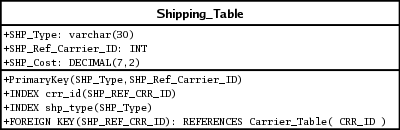
\includegraphics{Tables/ShippingTable.png}\\
        \\
        \subsection{Employee Management}

        The Employee Management section is actually two sections. There is the Employee portion which
        spans two tables, the Employee Table for employee information, and the Login Table which
        keeps track of the hours an employee works between logging in and out of the clients. The
        other section is the security aspect of the program as it relates to employees. It also spans
        two tables; the ACL Table and the Key Table.\\
        \\
        {\bf Employee Table}\\
        \\
        \\
        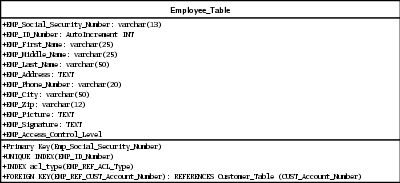
\includegraphics{Tables/EmployeeTable.png}
        \\
        \\
        The Employee Table keeps track of all pertinent information about employees that would
        be needed by an employer. Basic personal information such as First, Middle, and Last name
        as well as Contact information are maintained here. Each employee in the table has a unique
        employee identification number associated with them to avoid having to use the Social
        Security Number as a key. This also allows data such as the Social Security number to be
        encrypted to alleviate underprivileged users from seeing it. Each employee also has a
        field for a picture link and signature link to help with positive identification. The other
        field in this table is the password field which is used to store a users password to allow
        a user to login, and which is also used to decrypt the keys from the key table. Each user
        is also associated with a ACL entry in the ACL Table.\\
        \\
        {\bf Login Table}\\
        \\
        \\
        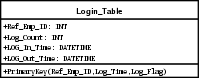
\includegraphics{Tables/LoginTable.png}\\
        \\
        \\
        The Login Table tracks the amount of time an employee has been logged in based on when
        they logged into their first client to when they logout of their last client. The structure
        is very simple. It references an employee ID and has a Count field. When the count is greater
        than zero the user is logged in and upon first entry a value will be inserted into the
        Log In Time field. When the value of Count reaches zero again a value will be inserted into
        the Log Out Time field.

        \subsection{Security}

        {\bf Access Control List Table}\\
        \\
        \\
        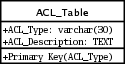
\includegraphics{Tables/ACL.png}\\
        \\
        \\
        The ACL table which is short for Access Control List Table manages which user types have access
        to different levels of program use. All this table contains is a Name of a user type and a description
        of their functionality. Currently we foresee only four user types and will likely not have an
        interface to manage this table.\\
        \\
        \\
        {\bf Key Table}\\
        \\
        \\
        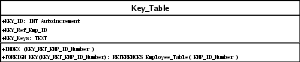
\includegraphics{Tables/KeyTable.png}\\
        \\
        \\
        The Key Table is used to manage the keys used to unencrypt the data stored in the database. The
        entry in this table will reference a valid user in the Employee Table and the text field will
        contain encrypted data that the user's password was used to encrypt. When the password is used
        to decrypt this data the user can obtain the keys used to encrypt global database data. A few
        example fields that are going to be stored as encrypted data are Credit Card Numbers and Expiration
        Date pairs as well as Social Security Numbers. This will add a level of database security that
        will prevent or deter malicious users from stealing valuable information from the database.\\
        \\

    \newpage

    \section{YardSale Client Application Design}
    The YardSale client is a modular structure designed to
    be flexible enough to accommodate any style of business.
    Each screen uses a bottom-oriented toolbar containing access
    to the on-screen calculator and keyboard, as well as the
    current time, an UNDO button, and a backwards navigation
    button.\\
    \subsection{Main Menu}
    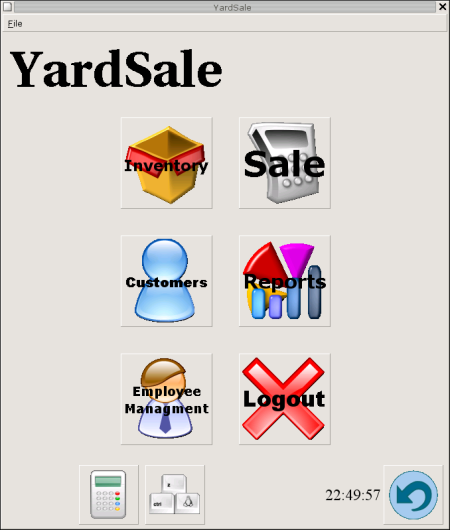
\includegraphics{ys_main_screener.png}\\

    The Main Menu is designed to allow users to quickly
    access any part of the YardSale client.  Buttons are available
    to users depending on access level.  The screen shown above
    displays an administrative user's access, as all options are
    currently available. The bottom toolbar does not contain the
    backwards navigation button, as this is the top-level screen.
    The buttons are enlarged to support touchscreen access.\\

    \subsection{Sales Screen}
    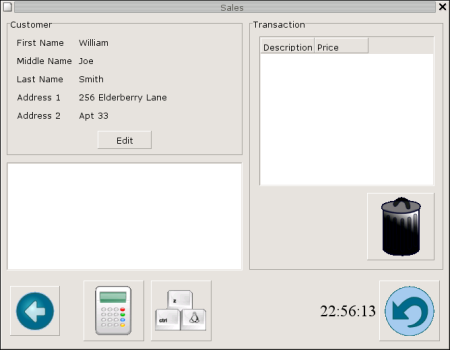
\includegraphics{ys_sales_screener.png}\\

    The Sales Screen is designed to provide much information and functionality, in
    an easy-access and user-friendly manner.  It displays
    information about the current customer, which may be edited to
    make any corrections or updates.  Below this is an inventory item
    list, which expands into a tree form to list similar
    products.  This section may be used in the case of a barcode
    scanner malfunction, or to give information about items similar
    to the ones being purchased.  To the right of the screen is the
    transaction shopping cart, which displays names and prices of
    items currently entered into the system to be purchased during this
    transaction.  When items are present in this list, a running
    total (including tax) is displayed at the bottom of the list.
    The trash can icon is used to remove unwanted items from the
    list.\\

    \subsection{Inventory Screen}
    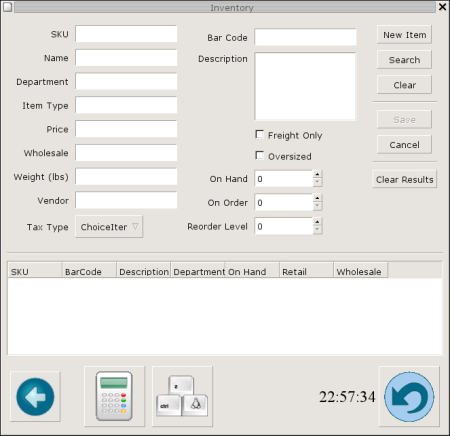
\includegraphics{ys_inv_screener.png}\\

    The Inventory Screen can display information pertaining to all
    inventory items currently stored in the database.  There are
    fields available for every possible value of an
    inventory item, which may be edited and saved.  In addition to these
    characteristics, the Inventory Screen has many other functions which it can perform.
    It can be used to add items to the inventory by filling in the
    appropriate fields and clicking the 'New Item' button.  The
    Search function is used by entering the desired information
    into the appropriate fields and clicking the 'Search' button.
    This will cause all inventory items present in the database
    that satisfy the criteria to be displayed in the window at the
    bottom of the screen.  For error checking purposes, a 'Save'
    and a 'Cancel' button are used when exiting this screen.  This
    screen should only be available to manager-access-level users
    and higher.\\

    \subsection{Employee Management Screen}
    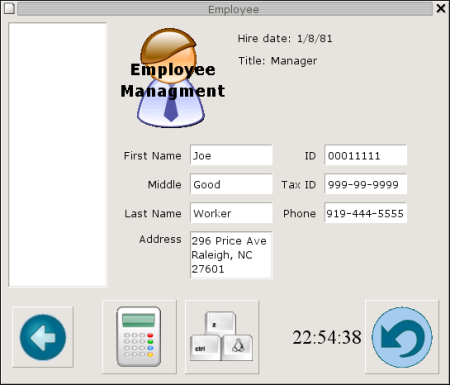
\includegraphics{ys_employee_screener.png}\\

    The Employee Management Screen is designed to store and
    display information pertaining to all employees currently in the
    system.  There are fields available for every possible value
    of an employee item in the database.  Information is displayed
    by entering the desired employee's ID number and pressing
    enter.  This screen should be carefully guarded, as sensitive
    information is displayed.  It should only be available to
    manager-access-level users and higher.\\

    \newpage

    \subsection{On-screen Calculator}
    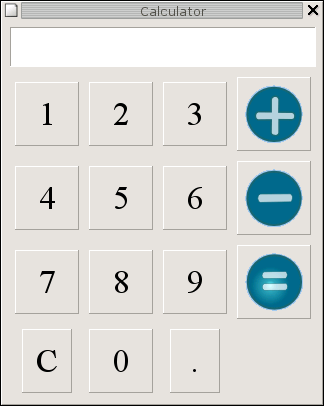
\includegraphics{ys_calc_screener.png}\\

    The On-Screen Calculator is designed to provide the user with
    an easy-access, user-friendly calculator and number pad.  It
    is available to all users from each screen in the system, via the tool bar
    at the bottom of the screen.  It provides the functionality of
    a basic calculator (add and subtract, multiply and divide to
    be added at a later date).  Numbers entered and the results
    are displayed in the box at the top of the calculator.\\

\chapter{Implementation}

    \section{Database Level Implementation}


        \subsection{Customer Management}
        {\tt\small
        DROP TABLE IF EXISTS Customer\_Table;\\

        CREATE TABLE Customer\_Table(
        \begin{list}{}
            \item{CUST\_Account\_Number INT AUTO\_INCREMENT NOT NULL,}
            \item{CUST\_First\_Name varchar(25),}
            \item{CUST\_Middle\_Name varchar(25),}
            \item{CUST\_Last\_Name varchar(50),}
            \item{CUST\_Address TEXT,}
            \item{CUST\_Phone varchar(20),}
            \item{CUST\_City varchar(50),}
            \item{CUST\_Zip varchar(12),}
            \item{CUST\_Credit\_Card\_Number varchar(20),}
            \item{CUST\_CC\_Exp\_Date varchar(6),}
            \item{CUST\_Name\_On\_CC TEXT,}
            \item{CUST\_Signature TEXT,}
            \item{CUST\_Photo TEXT,}
            \item{Primary Key(CUST\_Account\_Number)}
        \end{list}
        )type=InnoDB\\
        }

        \subsection{Inventory Management}
        {\tt\small
        DROP TABLE IF EXISTS Inventory\_Table;\\

        CREATE TABLE Inventory\_Table(
        \begin{list}{}
            \item{INV\_SKU\_Number                  varchar(10),}
            \item{INV\_Bar\_Code\_Number             varchar(30),}
            \item{INV\_Item\_Description            TEXT,}
            \item{INV\_Item\_Department             varchar(30),}
            \item{INV\_Quantity\_On\_Hand            INT,}
            \item{INV\_Quantity\_On\_Order           INT,}
            \item{INV\_Reorder\_Level               INT,}
            \item{INV\_Reorder\_Quantity            INT,}
            \item{INV\_Item\_Type                   varchar(20),}
            \item{INV\_REF\_TAX\_Tax\_Type            INT NOT NULL,}
            \item{INV\_REF\_VND\_Vendor\_ID           INT NOT NULL,}
            \item{INV\_Retail\_Price                DECIMAL(7,2),}
            \item{INV\_Wholesale\_Price             DECIMAL(7,2),}
            \item{INV\_Bulk\_Price                  TEXT,}
            \item{INV\_Date\_Last\_Received          DATETIME,}
            \item{INV\_Weight\_Pounds               FLOAT,}
            \item{INV\_Oversized\_Flag              enum('T','F'),}
            \item{INV\_Ship\_By\_Freight             enum('T','F'),}
            \item{INV\_Comment                     TEXT,}
            \item{Primary Key (INV\_SKU\_Number),}
            \item{UNIQUE INDEX (INV\_Bar\_Code\_Number),}
            \item{INDEX tax\_id (INV\_REF\_TAX\_Tax\_Type),}
            \item{INDEX vnd\_id (INV\_REF\_VND\_Vendor\_ID),}
            \item{FOREIGN KEY (INV\_REF\_TAX\_Tax\_Type)}
            \item{REFERENCES Tax\_Table(TAX\_ID),}
            \item{FOREIGN KEY (INV\_REF\_VND\_Vendor\_ID)}
            \item{REFERENCES Vendor\_Table(VND\_ID)}
        \end{list}
        ) type=InnoDB\\
        }

        {\tt\small
        DROP TABLE IF EXISTS Tax\_Table;\\

        CREATE TABLE Tax\_Table(
        \begin{list}{}
            \item{TAX\_ID          INT AUTO\_INCREMENT NOT NULL,}
            \item{TAX\_Name        varchar(20),}
            \item{TAX\_Percent     FLOAT,}
            \item{Primary Key (TAX\_ID)}
        \end{list}
        )type=InnoDB\\
        }

        \subsection{Transaction Handling}
        {\tt\small
        DROP TABLE IF EXISTS Transaction\_Log\_Table;\\

        CREATE TABLE Transaction\_Log\_Table(
        \begin{list}{}
            \item{TRANS\_REF\_EMP\_ID\_Number                 INT,}
            \item{TRANS\_REF\_INV\_SKU\_Number                varchar(10),}
            \item{TRANS\_REF\_CUST\_Account\_Number           INT,}
            \item{TRANS\_Sale\_Price                        DECIMAL(10,2),}
            \item{TRANS\_ID                                INT NOT NULL,}
            \item{TRANS\_Quantity                          INT,}
            \item{TRANS\_Comment                           TEXT,}
            \item{Primary Key(TRANS\_REF\_EMP\_ID\_Number,}
            \begin{list}{}
                \item{TRANS\_REF\_INV\_SKU\_Number,}
                \item{TRANS\_REF\_CUST\_Account\_Number,}
                \item{TRANS\_Sale\_Price, TRANS\_ID,}
                \item{TRANS\_Quantity),}
            \end{list}
            \item{INDEX trans\_id (TRANS\_ID),}
            \item{INDEX emp\_id (TRANS\_REF\_EMP\_ID\_Number),}
            \item{INDEX sku\_num (TRANS\_REF\_INV\_SKU\_Number),}
            \item{INDEX cust\_acct (TRANS\_REF\_CUST\_Account\_Number),}
            \item{FOREIGN KEY (TRANS\_REF\_EMP\_ID\_Number) REFERENCES Employee\_Table(EMP\_ID\_Number),}
            \item{FOREIGN KEY (TRANS\_REF\_INV\_SKU\_Number) REFERENCES Inventory\_Table(INV\_SKU\_Number),}
            \item{FOREIGN KEY (TRANS\_REF\_CUST\_Account\_Number) REFERENCES Customer\_Table(CUST\_Account\_Number)}
        \end{list}
        )type=InnoDB\\
        }

        {\tt\small
        DROP TABLE IF EXISTS Package\_Table;\\

        CREATE TABLE Package\_Table(
        \begin{list}{}
            \item{PKG\_ID\_Number                           INT AUTO\_INCREMENT NOT NULL,}
            \item{PKG\_REF\_TRANS\_ID                        INT,}
            \item{PKG\_REF\_CUST\_Account\_Number             INT,}
            \item{PKG\_REF\_CRR\_ID\_Number                   INT,}
            \item{PKG\_Tracking\_Number varchar(50),}
            \item{PKG\_REF\_SHP\_Shipping\_Type varchar(30),}
            \item{Primary Key(PKG\_ID\_Number),}
            \item{INDEX trans\_id (PKG\_REF\_TRANS\_ID),}
            \item{INDEX cust\_acct (PKG\_REF\_CUST\_Account\_Number),}
            \item{INDEX crr\_id (PKG\_REF\_CRR\_ID\_number),}
            \item{INDEX shp\_type (PKG\_REF\_SHP\_Shipping\_Type),}
            \item{FOREIGN KEY (PKG\_REF\_TRANS\_ID) REFERENCES Transaction\_Log\_Table( TRANS\_ID ),}
            \item{FOREIGN KEY (PKG\_REF\_CUST\_Account\_Number) REFERENCES Customer\_Table( CUST\_Account\_Number ),}
            \item{FOREIGN KEY (PKG\_REF\_CRR\_ID\_Number) REFERENCES Carrier\_Table( CRR\_ID ),}
            \item{FOREIGN KEY (PKG\_REF\_SHP\_Shipping\_Type) REFERENCES Shipping\_Table( SHP\_Type )}
        \end{list}
        ) type=InnoDB\\
        }

        {\tt\small
        DROP TABLE IF EXISTS Carrier\_Table;\\

        CREATE TABLE Carrier\_Table(
        \begin{list}{}
            \item{CRR\_ID                          INT AUTO\_INCREMENT NOT NULL,}
            \item{CRR\_Name                        varchar(50),}
            \item{CRR\_Pickup\_Location             TEXT,}
            \item{CRR\_Phone\_Number                varchar(20),}
            \item{Primary Key (CRR\_ID)}
        \end{list}
        )type=InnoDB\\
        }

        {\tt\small
        DROP TABLE IF EXISTS Shipping\_Table;\\

        CREATE TABLE Shipping\_Table(
        \begin{list}{}
            \item{SHP\_Type                varchar(30),}
            \item{SHP\_REF\_CRR\_ID          INT,}
            \item{SHP\_Cost                DECIMAL(7,2),}
            \item{Primary Key(SHP\_Type, SHP\_REF\_CRR\_ID, SHP\_Cost),}
            \item{INDEX crr\_id (SHP\_REF\_CRR\_ID ),}
            \item{INDEX shp\_type (SHP\_Type),}
            \item{FOREIGN KEY (SHP\_REF\_CRR\_ID) REFERENCES Carrier\_Table( CRR\_ID )}
        \end{list}
        )type=InnoDB\\
        }

        \subsection{Employee Management}
        {\tt\small
        DROP TABLE IF EXISTS Employee\_Table;\\

        CREATE TABLE Employee\_Table(
        \begin{list}{}
            \item{EMP\_Social\_Security\_Number             varchar(13) NOT NULL,}
            \item{EMP\_ID\_Number                           INT NOT NULL,}
            \item{EMP\_First\_Name                          varchar(25),}
            \item{EMP\_Middle\_Name                         varchar(25),}
            \item{EMP\_Last\_Name                           varchar(50),}
            \item{EMP\_Address                              TEXT,}
            \item{EMP\_Phone\_Number                        varchar(20),}
            \item{EMP\_City                                 varchar(50),}
            \item{EMP\_Zip                                  varchar(12),}
            \item{EMP\_Picture                              TEXT,}
            \item{EMP\_Signature                            TEXT,}
            \item{EMP\_REF\_ACL\_Type                       varchar(30),}
            \item{\#EMP\_REF\_CUST\_Account\_Number            INT,}
            \item{Primary Key (EMP\_Social\_Security\_Number),}
            \item{UNIQUE INDEX(EMP\_ID\_Number),}
            \item{INDEX acl\_type (EMP\_REF\_ACL\_Type),}
            \item{\#INDEX acct\_number (EMP\_REF\_CUST\_Account\_Number),}
            \item{FOREIGN KEY (EMP\_REF\_ACL\_Type) REFERENCES ACL\_Table(ACL\_Type),}
            \item{\#FOREIGN KEY (EMP\_REF\_CUST\_Account\_Number) REFERENCES Customer\_Table(CUST\_Account\_Number)}
        \end{list}
        ) type=InnoDB\\
        }

        {\tt\small
        DROP TABLE IF EXISTS Key\_Table;\\

        CREATE TABLE Key\_Table(
        \begin{list}{}
            \item{KEY\_ID                          INT AUTO\_INCREMENT,}
            \item{KEY\_REF\_EMP\_ID\_Number        INT,}
            \item{KEY\_Keys                        TEXT,}
            \item{PRIMARY KEY ( KEY\_ID ),}
            \item{INDEX ( KEY\_REF\_EMP\_ID\_Number ),}
            \item{FOREIGN KEY (KEY\_REF\_EMP\_ID\_Number) REFERENCES Employee\_Table( EMP\_ID\_Number )}
        \end{list}
        )type=InnoDB\\
        }

        {\tt\small
        DROP TABLE IF EXISTS ACL\_Table;\\

        CREATE TABLE ACL\_Table(
        \begin{list}{}
            \item{ACL\_Type varchar(30),}
            \item{ACL\_Description TEXT,}
            \item{Primary Key (ACL\_Type)}
        \end{list}
        ) type=InnoDB\\
        }

    \section{Application Level Implementation}

        \subsection{YardCalc}
        YardCalc is a generic on-screen calculator the user employs to
        enter prices.  This calculator uses a stack-based method of
        storing numbers and operators.\\
        {\sl SEE YARDSALE IMPLEMENTATION MANUAL SECTION 7.3}

        \subsection{YardDatabase}
        YardDatabase is the main database backend which does all
        translation from OO calls to SQL/ODBC.\\
        {\sl SEE YARDSALE IMPLEMENTATION MANUAL SECTION 7.6}

        \subsection{YardDBType}
        YardBDType is the abstract base class for all database
        objects.  All database types are assignable and contain a
        ToString() method to format the DB type to text.\\
        {\sl SEE YARDSALE IMPLEMENTATION MANUAL SECTION 7.8}

            \subsubsection{YardEmployeeType}
            YardEmployeeType is a subclass of YardDBType, which
            represents an employee record and contains functions for
            all possible items.\\
            {\sl SEE YARDSALE IMPLEMENTATION MANUAL SECTION 7.11}

            \subsubsection{YardInvType}
            YardInvType is a subclass of YardDBType, which
            represents an employee record and contains functions for
            all possible items.\\
            {\sl SEE YARDSALE IMPLEMENTATION MANUAL SECTION 7.15}
            \begin{list}{}
                \item {\bf YardInvType::BulkPricing}\\BulkPricing is a
                C++ structure that associates a quantity with a
                percentage for bulk pricing.\\
                {\sl SEE YARDSALE IMPLEMENTATION MANUAL SECTION 7.16}
            \end{list}

        \subsection{YardEmployee}
        YardEmployee is the employee management screen.  Depending on
        access level, users may insert/modify employee information via
        this screen.\\
        {\sl SEE YARDSALE IMPLEMENTATION MANUAL SECTION 7.10}

        \subsection{YardInventory}
        YardInventory is the inventory management screen, which allows
        searching.  Depending on access level, users may add inventory
        via the "New Item" button on this screen.\\
        {\sl SEE YARDSALE IMPLEMENTATION MANUAL SECTION 7.14}

        \subsection{YardException}
        YardException is the exception class from Crypto++.\\
        {\sl SEE YARDSALE IMPLEMENTATION MANUAL SECTION 7.12}

        \subsection{YardLog}
        YardLog is the logging widget, based on wxListCtrl and wxLog.
        This widget resets the default logging system and redirects
        all output to itself.  Different icons represent what type of
        log message is being displayed.\\
        {\sl SEE YARDSALE IMPLEMENTATION MANUAL SECTION 7.17}

        \subsection{YardLogin}
        YardLogin is the customized login screen.  The user will be
        asked for a username and password.  Also, a quick select icon
        will allow the user to rapidly select his/her name.\\
        {\sl SEE YARDSALE IMPLEMENTATION MANUAL SECTION 7.18}

        \subsection{YardMain}
        YardMain is the main menu screen, which displays graphical
        buttons for accessing each part of the system.\\
        {\sl SEE YARDSALE IMPLEMENTATION MANUAL SECTION 7.19}

        \subsection{YardSale}
        YardSale is the main application object, which returns a
        reference to a YardDatabase object.\\
        {\sl SEE YARDSALE IMPLEMENTATION MANUAL SECTION 7.20}

        \subsection{YardSaleScreen}
        YardSaleScreen is main sale screen, which contains the current
        transaction information and an interface to add new items to
        the transaction.  The payment screen can be accessed from
        YardSaleScreen.\\
        {\sl SEE YARDSALE IMPLEMENTATION MANUAL SECTION 7.21}

        \subsection{YardSplash}
        YardSplash is an eye-candy, startup splash screen that shows a
        progress bar.\\
        {\sl SEE YARDSALE IMPLEMENTATION MANUAL SECTION 7.22}

\chapter{Test Plan}
The YardSale system is tested constantly throughout the
development process.  These tests are administered through two
different methods: passive (automatic) testing, and active (user)
testing.

    \section{Passive Testing}

    The passive testing of YardSale is accomplished by our auto build system.  The auto build system pulls the latest source
    code from the repository and compiles it with the most strict settings.  If the code fails the system reports the error
    on our website.  The auto build system will also compile the code on six other architechures including Amd64, Sparc, Mac OSX,
    Linux, and Microsoft Windows.  The extensive compilation of the source code ensures that no platform dependant source code
    violates the portability of the project.

    \section{Active Testing}
    There are several methods which are utilized by our
    development team to manually test the YardSale system
    throughout the development process.
        \subsection{Testing Mains}
        Each non-gui object in the YardSale system has an integrated main loop which allows the program to build test versions of
        each of the objects.  These test objects then execute a series of tests to ensure that the object is working exactly to specification.
        If any of these tests fail the system will report the exact location of the failure.

        \subsection{Warm-Body Testing}
        Each GUI screen is tested by our virtual employees for both functionality and usability.  The employees report back to the developers with any
        bugs they find through our bug tracking system.  We also have weekly usability conferences where we discuss the merits of a particular interface.

        \subsection{Verbose Program Information}
        YardSale is designed to report back a large amount of valuable debug information to the developer and to keep the non-technical user
        informed about the status of the program.  YardSale uses exceptions to ensure that single functions cannot violate the integrity of the system
        on a global level.  In addition, all database interfaces have special logging information that reports the exact status of all database calls; this
        allows the developers to get instant access to valuable SQL and connection results.

\end{document}
